\section{Problem Statement}

The problem we attempted to solve is that existing CAD programs are not designed for laser cutting. Laser cutting requires 2D schematics so non-parametric drawing programs are appealing to use but laser cutters produce 3D objects so parametric design capabilities are highly desirable. Parametric design is based on setting constraints and dimensions (the way an engineer would design). This approach facilitates creating real objects. The need for parametric design and basic drawing capabilities results in users switching between a variety of programs which each offer some subset of desired features. Consequently users often find themselves switching back and forth between programs when creating designs. This issue with the current laser cutting workflow is depicted in Figure~\ref{fig:laserCuttingWorkflow}. A user creates the skeleton for a design in a parametric CAD program intended for modeling 3D objects (such as Onshape, Fusion360, or Solidworks). The user then imports this design into a some vector drawing software (Adobe Illustrator or CorelDRAW), then into a program capable of producing tool-paths (in this case CorelDRAW), which are finally sent to the laser cutter.

\begin{figure}[!h]
  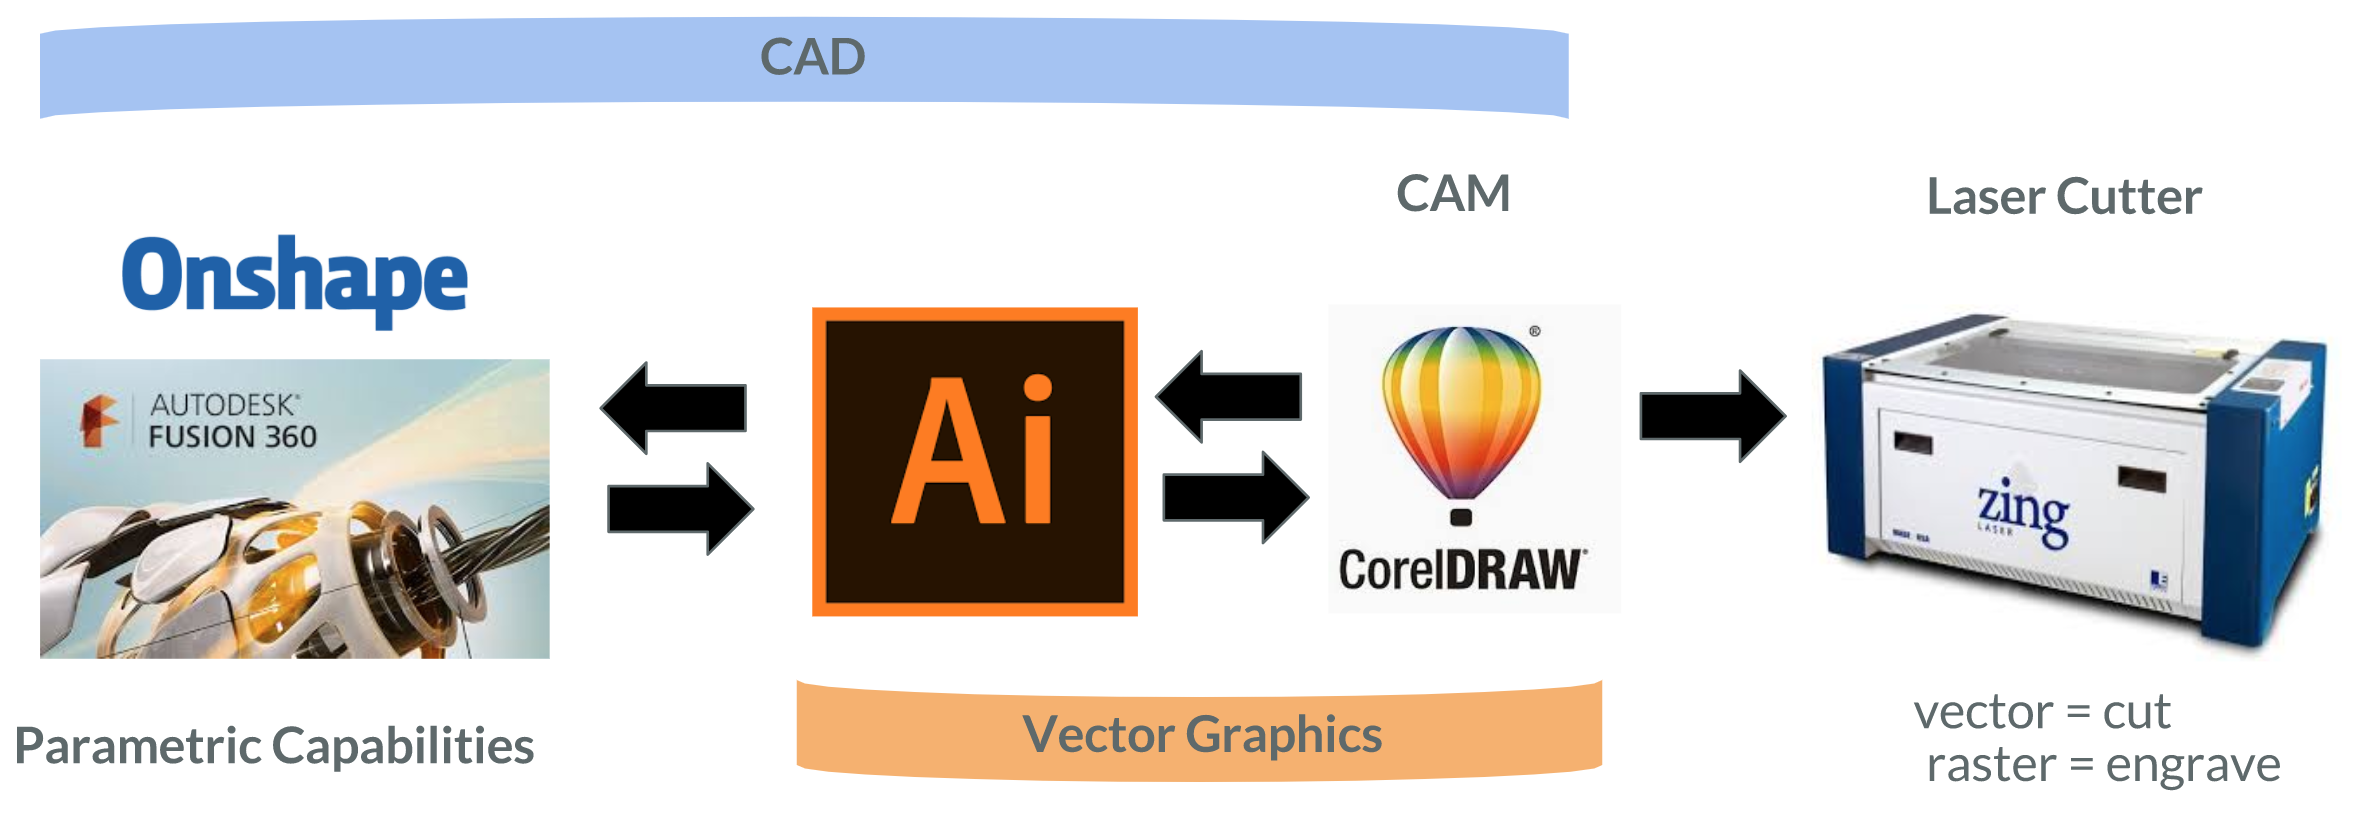
\includegraphics[width=\linewidth]{laserCuttingWorkflow.jpg}
  \caption{The current laser cutting workflow. Notice the ``pong effect" between design programs in the CAD portion of the workflow.}
  \label{fig:laserCuttingWorkflow}
\end{figure}


Another issue with the current laser cutting workflow is the price and complexity of commercial CAD software. Be it parametric CAD - Onshape, Fusion360, Solidworks - or visual design software - the Adobe Suite, CorelDRAW - commercial design software often requires a user pay regular subscription fees or retains ownership over user produced data. This makes laser cutting inaccessible to new hobbyists who may be unwilling to pay the fees or concerned with privacy of files they create. Additionally existing CAD software is over-engineered and inappropriate for a majority laser cutting tasks. most parametric CAD programs also incorporate sculpting and constructive solid geometry (CSG) tools which are completely irrelevant to a user interested in laser cutting. Likewise visual design programs involve complex layering systems and style modification tools with no relevance to physical designs. An ideal CAD program for laser cutting would incorporate features of both traditional drawing programs and parametric design programs. Our goal was to create a single-page web-based program specifically designed for laser cutting. A program that combined the best parts of 2D drawing programs and 3D CAD programs, while leaving the unnecessary parts behind. Specifically, we wanted our program to be SVG based so that drawings could be easily sent to a laser cutter, and we wanted to incorporate a geometric constraint solver so that we could easily create real-world objects. The laser cutting workflow we would ultimately want to create would involve one program for producing all designs and tool paths. This is depicted in Figure~\ref{fig:2to3DWorkflow}.

\begin{figure}[h]
  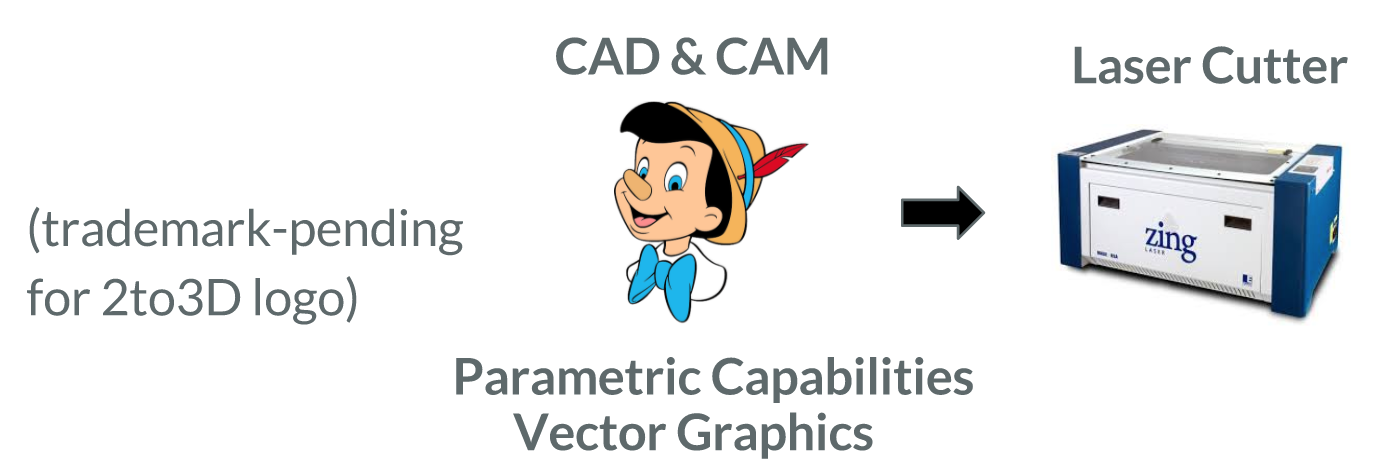
\includegraphics[width=\linewidth]{2to3DWorkflow.jpg}
  \caption{The laser cutting workflow we aim to create.}
  \label{fig:2to3DWorkflow}
\end{figure}

Semester time constraints meant we did not incorporate CAM or engraving features into 2to3D.